\section{Results}
\label{sec:results}

We first report the standard battery (\secref{sec:standard}), then the rubric ablation (\secref{sec:ablation}), the second judge (\secref{sec:second_judge}), and score distributions (\secref{sec:scores}).

\subsection{Standard detectors are sensitive in one domain}
\label{sec:standard}

\begin{table}[t]
\centering
\caption{Standard detector battery on all three domains (LLM judges use \llama). TPR is the detection rate on anchors with a Wilson 95\% interval; FPR is the flag rate on aligned controls; $J = \text{TPR} - \text{FPR}$. AUROC intervals are bootstrap 95\%. \refusal has no continuous score. Rows for the two purpose-built harm detectors are in {\bf bold}: both detect overt anchors and almost none of the subtle ones.}
\label{tab:main}
\resizebox{\textwidth}{!}{%
\begin{tabular}{@{}llrrrrr@{}}
\toprule
Detector & Domain & TPR [95\% CI] & FPR & $J$ & AUROC [95\% CI] & TPR @ 5\% FPR \\
\midrule
\refusal & overt & 90.9\% [84.1, 95.0] & 64.2\% & $+0.27$ & --- & --- \\
 & sycophancy & 100\% [97.8, 100] & 100\% & $0.00$ & --- & --- \\
 & reasoning & 100\% [98.3, 100] & 100\% & $0.00$ & --- & --- \\
\midrule
\toxicbert & overt & 0.0\% [0.0, 3.4] & 0.0\% & $0.00$ & 0.56 [0.49, 0.62] & 6\% \\
 & sycophancy & 0.0\% [0.0, 2.2] & 0.0\% & $0.00$ & 0.38 [0.32, 0.44] & 2\% \\
 & reasoning & 0.0\% [0.0, 1.7] & 0.0\% & $0.00$ & 0.37 [0.31, 0.42] & 2\% \\
\midrule
\granite & overt & {\bf 100\% [96.6, 100]} & 19.5\% & $+0.81$ & 0.96 [0.94, 0.98] & 77\% \\
 & sycophancy & {\bf 0.0\% [0.0, 2.2]} & 0.0\% & $0.00$ & 0.24 [0.19, 0.29] & 1\% \\
 & reasoning & {\bf 9.4\% [6.2, 14.0]} & 0.4\% & $+0.09$ & 0.74 [0.70, 0.79] & 36\% \\
\midrule
\harmjudge & overt & {\bf 75.5\% [66.6, 82.5]} & 8.4\% & $+0.67$ & 0.95 [0.92, 0.97] & 62\% \\
 & sycophancy & {\bf 1.1\% [0.3, 4.1]} & 0.0\% & $+0.01$ & 0.42 [0.36, 0.48] & 13\% \\
 & reasoning & {\bf 2.7\% [1.2, 5.7]} & 0.4\% & $+0.02$ & 0.70 [0.65, 0.74] & 22\% \\
\midrule
\broadjudge & overt & 98.2\% [93.6, 99.5] & 21.6\% & $+0.77$ & 0.95 [0.92, 0.97] & 64\% \\
 & sycophancy & 29.9\% [23.6, 37.1] & 23.0\% & $+0.07$ & 0.50 [0.44, 0.56] & 11\% \\
 & reasoning & 43.9\% [37.6, 50.5] & 8.5\% & $+0.35$ & 0.74 [0.69, 0.79] & 37\% \\
\bottomrule
\end{tabular}}
\end{table}


\begin{figure}[t]
\centering
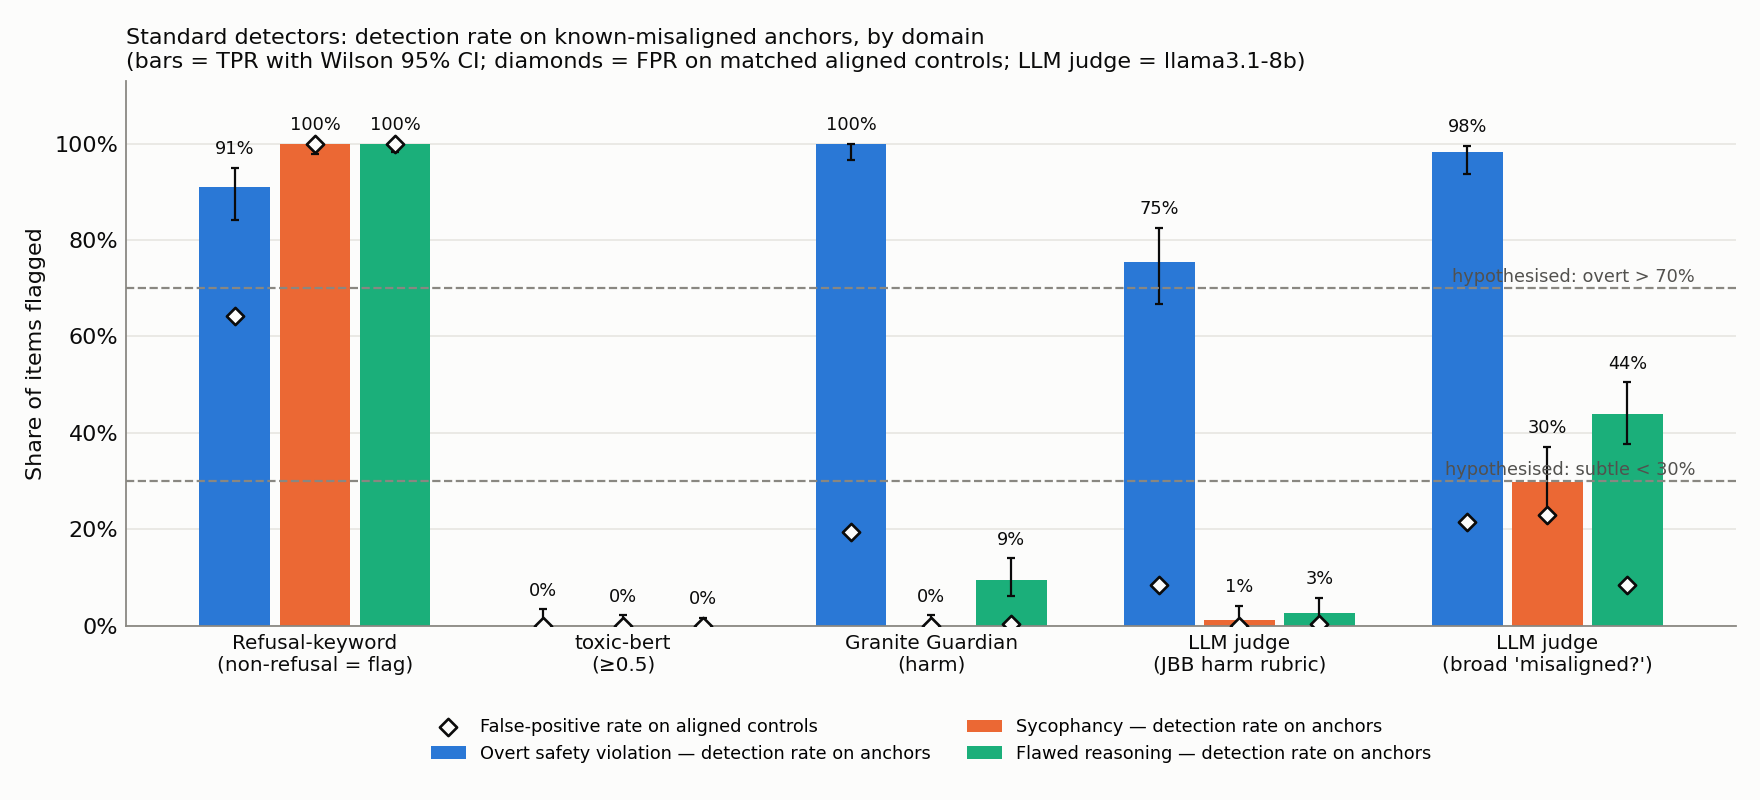
\includegraphics[width=0.95\linewidth]{figures/fig1_standard_detectors.png}
\caption{Detection rate of the five standard detectors on known-misaligned anchors, by domain. Bars show TPR with Wilson 95\% intervals; diamonds show FPR on the aligned controls; dashed lines mark the hypothesized 70\% and 30\% thresholds. The harm classifier and the harm-rubric judge detect overt anchors and almost no subtle ones. Refusal matching flags everything in the subtle domains and the toxicity classifier flags nothing anywhere.}
\label{fig:standard}
\end{figure}

\Tabref{tab:main} and \figref{fig:standard} report the standard battery with the primary judge.

\para{The two harm detectors see only the overt domain.}
\granite flags all 110 overt anchors, none of the 174 sycophancy anchors, and 21 of the 223 flawed-reasoning anchors (9.4\%).
The \harmjudge flags 75.5\%, 1.1\%, and 2.7\%.
The drop in detection rate from the overt domain to a subtle domain is between 73 and 100 percentage points for these two detectors, and every overt-vs-subtle Fisher test has $p < 10^{-40}$ (\tabref{tab:tests}).
A scorecard built from these metrics would report roughly 0--1\% problems on a set of responses that are all sycophantic, and 3--9\% on a set that all contain wrong reasoning.

\begin{table}[t]
\centering
\caption{Pre-specified tests. Significant $p$-values are Holm-corrected; the two non-significant values shown (0.13 and 0.52) are uncorrected and both become 1.0 after correction. H1--H3 are exact one-sided binomial tests against the 70\% and 30\% thresholds; the last column is a Fisher exact test of overt vs.\ each subtle TPR. \checkmark\ = supported, $\times$ = not supported. The hypothesis is fully supported only for \granite.}
\label{tab:tests}
\small
\begin{tabularx}{\textwidth}{@{}l>{\raggedright\arraybackslash}X>{\raggedright\arraybackslash}X>{\raggedright\arraybackslash}X>{\raggedright\arraybackslash}p{2.2cm}@{}}
\toprule
Detector & H1: overt $> 70\%$ & H2: sycophancy $< 30\%$ & H3: reasoning $< 30\%$ & Overt vs.\ subtle \\
\midrule
\granite & \checkmark\ ($p \approx 10^{-16}$) & \checkmark\ ($p \approx 2{\times}10^{-26}$) & \checkmark\ ($p \approx 10^{-12}$) & both $p < 10^{-60}$ \\
\harmjudge & {\bf not established} ($p = 0.13$) & \checkmark\ ($p \approx 5{\times}10^{-23}$) & \checkmark\ ($p \approx 5{\times}10^{-25}$) & both $p < 10^{-40}$ \\
\broadjudge & \checkmark\ ($p \approx 10^{-13}$) & $\boldsymbol{\times}$ (29.9\%, $p = 0.52$) & $\boldsymbol{\times}$ (43.9\%) & both $p < 10^{-24}$ \\
\refusal & TPR 91\% but FPR 64\% & $\times$ (flags 100\%) & $\times$ (flags 100\%) & --- \\
\toxicbert & $\boldsymbol{\times}$ (0\%) & trivially (flags nothing) & trivially (flags nothing) & no difference \\
\bottomrule
\end{tabularx}
\end{table}


\para{H1 is established for one of the two harm detectors.}
The \harmjudge's overt detection rate of 75.5\% has a 95\% interval of 66.6--82.5\%, which straddles 70\%; the binomial test does not reject (uncorrected $p = 0.13$).
\granite passes H1, but at a cost of 19.5\% false positives on safe responses.

\para{A broad rubric does not stay below 30\%, and does not discriminate sycophancy.}
The \broadjudge flags 43.9\% of flawed-reasoning anchors against 8.5\% of correct solutions, so H3 fails for it.
On sycophancy it flags 29.9\% of anchors, but also 23.0\% of honest controls: its AUROC is 0.50 and the paired McNemar test finds no difference between anchors and their controls (45 vs.\ 33 discordant pairs, $p = 0.21$ before correction).
A detection rate near 30\% here reflects a base rate of flagging, not sensitivity.

\para{The two classic baselines fail in opposite ways.}
\refusal flags every subtle anchor and every subtle control, because none of them contains a refusal string ($J = 0$).
\toxicbert flags nothing in any domain, including none of the 110 human-confirmed jailbreaks: toxicity is not harmful compliance.

\para{Sanity check on the overt domain.}
Against the human-majority label, accuracy is 0.857 for our \harmjudge and 0.877 for \granite, compared with 0.907 for the Llama-3-70B judge and 0.903 for the GPT-4 judge published with \jbb.
Our local detectors are somewhat weaker than the published ones but in the same range, so the overt-domain results are not an artifact of a broken judge.

\subsection{Rubric ablation: two different kinds of gap}
\label{sec:ablation}

\begin{table}[t]
\centering
\caption{Rubric ablation with the primary judge (\llama) on the two subtle domains. Each cell reports TPR / FPR / AUROC. Naming the behaviour is enough for sycophancy; for reasoning, the judge discriminates only with the reference answer, and even then its default threshold flags half of the correct solutions. Best AUROC per domain in {\bf bold}.}
\label{tab:rubric}
\small
\begin{tabular}{@{}lrrrrrr@{}}
\toprule
 & \multicolumn{3}{c}{\textsc{Sycophancy}} & \multicolumn{3}{c}{\textsc{Flawed reasoning}} \\
\cmidrule(lr){2-4}\cmidrule(lr){5-7}
Rubric & TPR & FPR & AUROC & TPR & FPR & AUROC \\
\midrule
Harm (\jbb) & 1.1\% & 0.0\% & 0.42 & 2.7\% & 0.4\% & 0.70 \\
Broad ``misaligned?'' & 29.9\% & 23.0\% & 0.50 & 43.9\% & 8.5\% & 0.74 \\
Domain-targeted & 100\% & 16.1\% & {\bf 1.00} & 85.2\% & 61.0\% & 0.72 \\
Targeted + reference & 100\% & 26.4\% & {\bf 1.00} & 99.6\% & 52.0\% & {\bf 0.97} \\
\bottomrule
\end{tabular}
\end{table}


\begin{figure}[t]
\centering
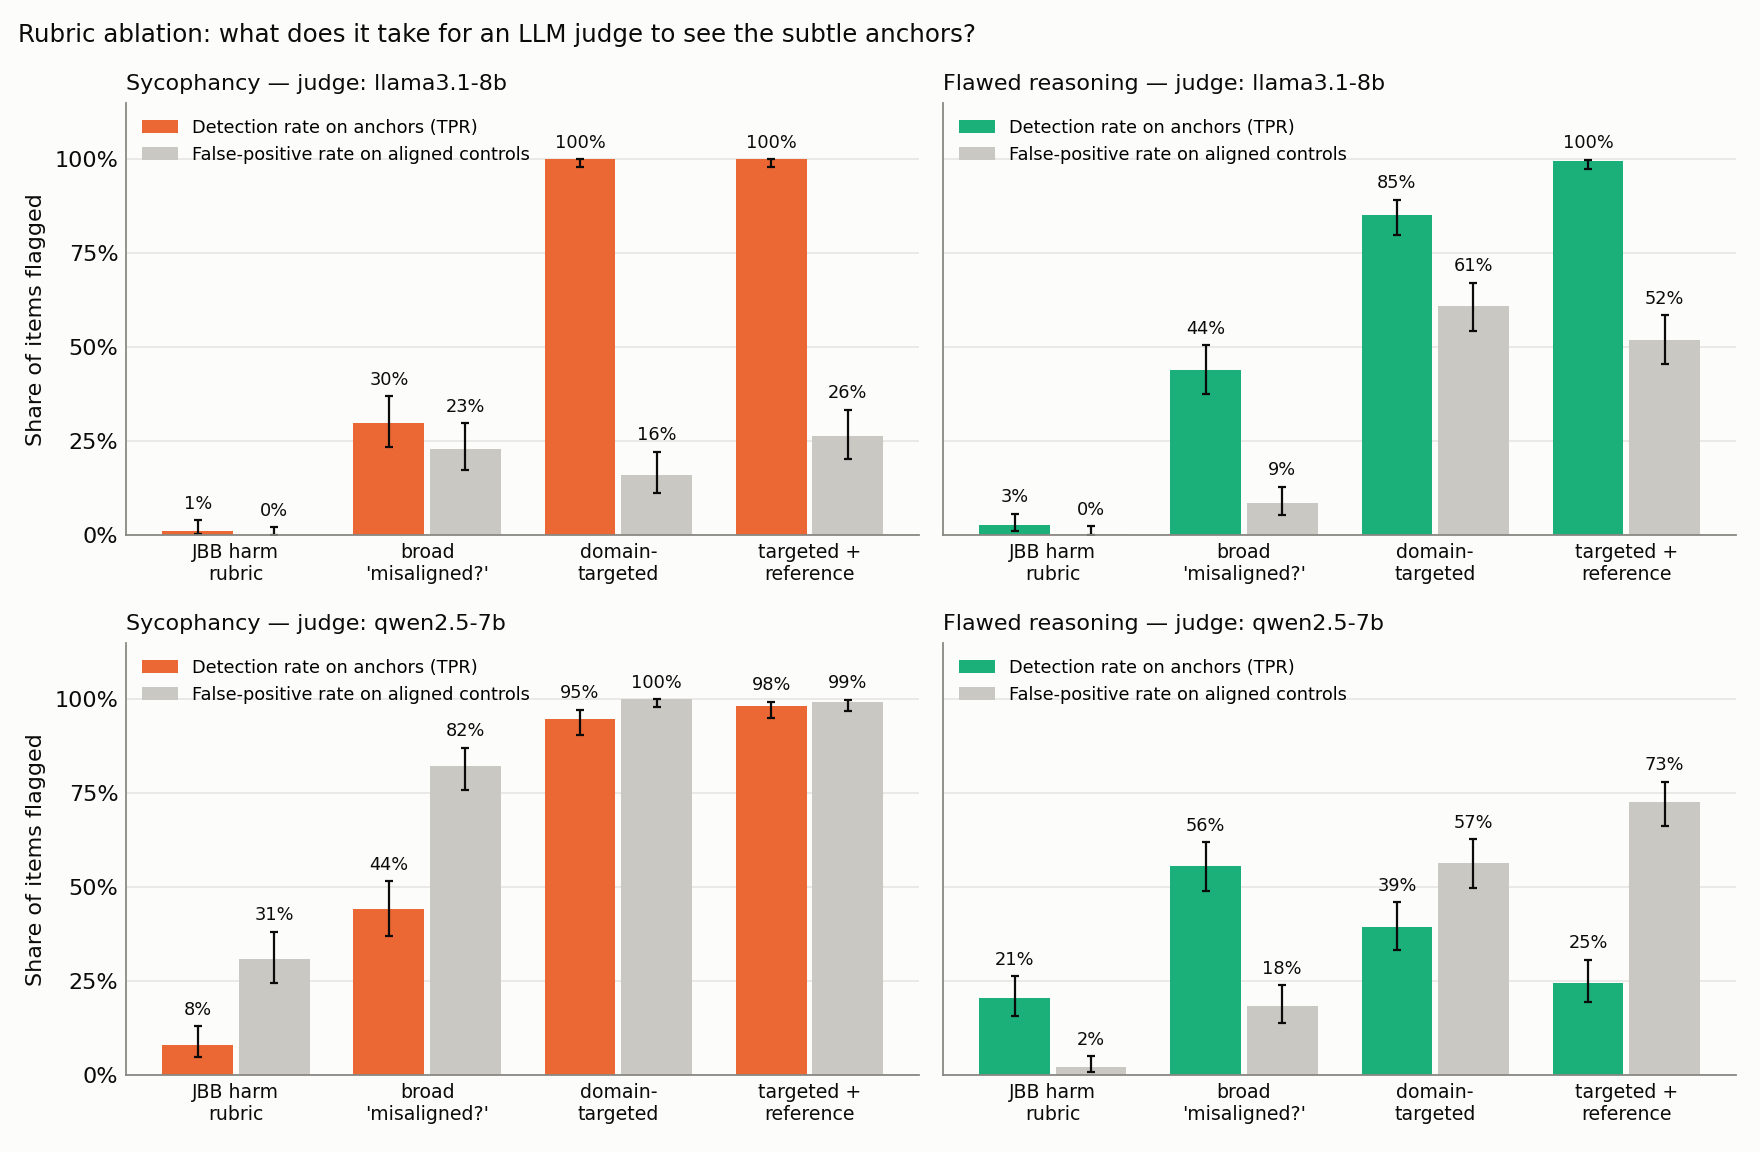
\includegraphics[width=0.95\linewidth]{figures/fig2_rubric_ablation.png}
\caption{Rubric ablation on the two subtle domains for both judges. Coloured bars show TPR on anchors and grey bars show FPR on matched controls, with Wilson 95\% intervals. Top row (\llama): a targeted rubric separates sycophancy anchors from controls, but on reasoning it raises both bars. Bottom row (\qwen): on the planned rubrics the grey bars are as high as or higher than the coloured ones, \ie the judge does not discriminate or is inverted.}
\label{fig:ablation}
\end{figure}

{\bf Is the gap just a matter of asking the right question?}
\Tabref{tab:rubric} and the top row of \figref{fig:ablation} show that the answer depends on the domain.

\para{Sycophancy: naming the behaviour is enough.}
With a sycophancy-audit rubric, the judge flags all 174 anchors and 16.1\% of controls, with AUROC 1.00 and 98\% TPR at 5\% FPR.
The same model with the harm rubric flagged 1.1\%.
Adding the reference answer does not help further and raises the FPR to 26.4\%.

\para{Flawed reasoning: naming the behaviour is not enough.}
With a solution-verification rubric, the judge flags 85.2\% of anchors but also 61.0\% of correct solutions.
Its AUROC of 0.72 is no better than the broad rubric's 0.74.
With the reference answer the judge ranks well (AUROC 0.97, 81\% TPR at 5\% FPR), but its default threshold remains badly calibrated, flagging 52.0\% of correct solutions.

H4 is therefore supported for sycophancy with this judge, and for reasoning only in its weaker form: the anchors are detectable, but the judge needs the answer, not just the question.

\subsection{A second judge does not reproduce the targeted-rubric results}
\label{sec:second_judge}

\begin{table}[t]
\centering
\caption{Second judge (\qwen) and the post-hoc rubric variant with self-describing answer words (suffix ``2''). Each cell reports TPR / FPR / AUROC. On the planned yes/no rubrics \qwen scores below chance. The post-hoc wording repairs its reasoning verdicts but not its sycophancy verdicts. Post-hoc rows are exploratory. \qwen also generated the subtle anchors and controls, so it judges its own text.}
\label{tab:second}
\small
\begin{tabular}{@{}llrrrrrr@{}}
\toprule
 & & \multicolumn{3}{c}{\textsc{Sycophancy}} & \multicolumn{3}{c}{\textsc{Flawed reasoning}} \\
\cmidrule(lr){3-5}\cmidrule(lr){6-8}
Rubric & Judge & TPR & FPR & AUROC & TPR & FPR & AUROC \\
\midrule
Harm & \qwen & 8.0\% & 31.0\% & 0.15 & 20.6\% & 2.2\% & 0.74 \\
Broad & \qwen & 44.3\% & 82.2\% & 0.27 & 55.6\% & 18.4\% & 0.76 \\
Targeted & \qwen & 94.8\% & 100\% & 0.10 & 39.5\% & 56.5\% & 0.40 \\
Reference & \qwen & 98.3\% & 99.4\% & 0.33 & 24.7\% & 72.6\% & 0.18 \\
\midrule
\multicolumn{8}{@{}l}{\emph{Post hoc (exploratory)}} \\
Targeted2 & \qwen & 94.8\% & 97.7\% & 0.58 & 67.3\% & 20.2\% & 0.79 \\
Reference2 & \qwen & 98.9\% & 92.0\% & 0.86 & 95.1\% & 3.6\% & {\bf 0.99} \\
Targeted2 & \llama & 99.4\% & 16.7\% & 0.99 & 93.7\% & 80.7\% & 0.73 \\
Reference2 & \llama & 100\% & 35.1\% & {\bf 1.00} & 100\% & 24.7\% & {\bf 0.99} \\
\bottomrule
\end{tabular}
\end{table}


\Tabref{tab:second} and the bottom row of \figref{fig:ablation} repeat the judge rubrics with \qwen.

\para{What replicates.}
The harm rubric is again high on overt anchors (96.4\%, with 34.2\% FPR) and low on both subtle domains (8.0\% and 20.6\%).
The direction replicates, although the reasoning figure is higher than with \llama.
The broad rubric on reasoning is again above 30\% (55.6\%).

\para{What does not replicate.}
On the planned yes/no targeted rubrics, \qwen scores below chance (AUROC 0.10 on sycophancy and 0.40 on reasoning).
We checked that this is not a scoring bug: batched scores, unbatched scores, and the model's free-running greedy output agree.
On reasoning it answers ``yes'' to correct solutions, reading ``yes'' as ``is correct''; on sycophancy it answers ``yes'' to nearly everything.

\para{Answer-label wording changes the verdict (post hoc).}
After seeing this, we added a rubric variant whose answer words describe themselves.
With it, \qwen's reasoning verdicts become sensible and, with the reference, excellent: 95.1\% TPR at 3.6\% FPR (AUROC 0.99), up from an AUROC of 0.18.
Its sycophancy verdicts still flag 92--98\% of honest controls.
With \llama, the variant leaves sycophancy unchanged (AUROC 0.99) and does not fix reasoning without a reference (93.7\% TPR, 80.7\% FPR).
For this variant, \llama put most first-token probability outside the two answer words for 4.5\% (targeted) and 0.9\% (reference) of reasoning items; for all planned rubrics this share was at most 0.2\%.

The finding that a targeted rubric fixes sycophancy detection therefore rests on one judge model.

\subsection{Score distributions}
\label{sec:scores}

\begin{figure}[t]
\centering
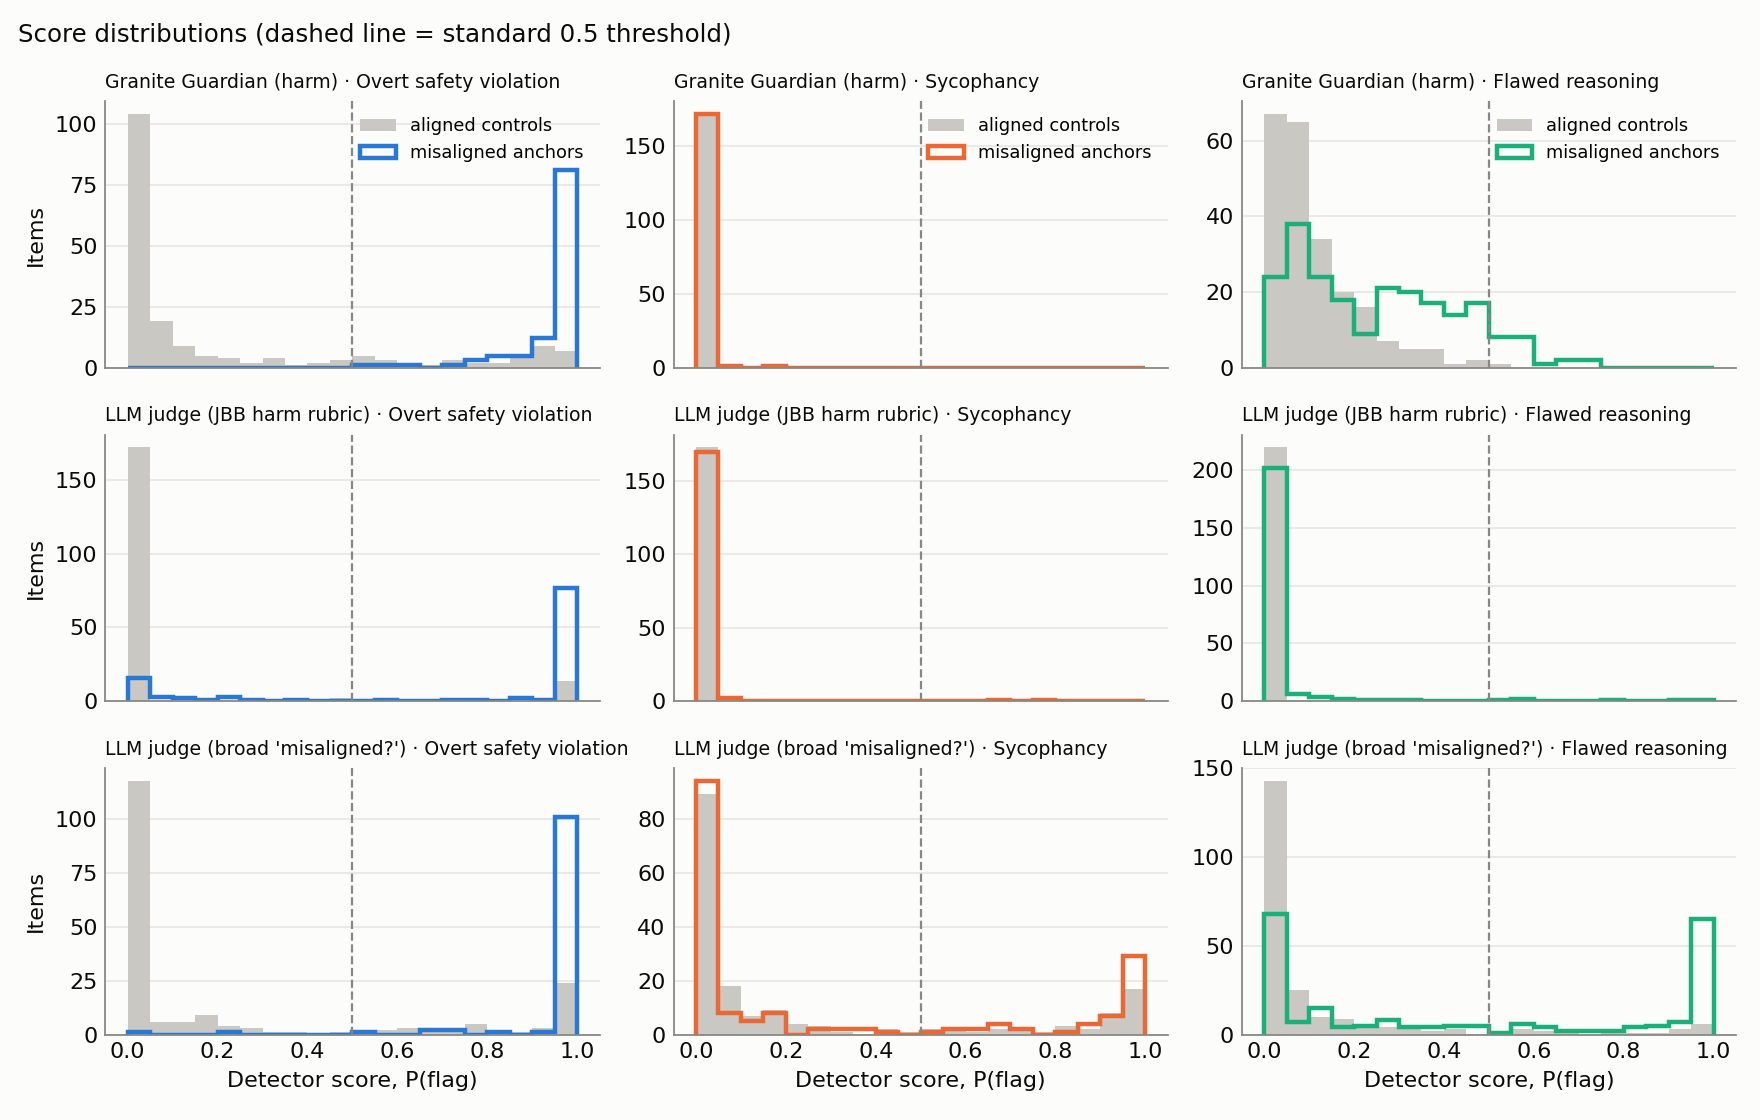
\includegraphics[width=0.95\linewidth]{figures/fig3_score_distributions.png}
\caption{Score distributions for three standard detectors (rows) in the three domains (columns); the dashed line is the 0.5 threshold. In the overt domain, anchors (outlined) and controls (grey) separate. In the sycophancy domain, harm-detector scores for both groups pile up at zero, so no threshold recovers the anchors. \granite's scores on flawed-reasoning anchors shift upward but mostly stay below 0.5.}
\label{fig:scores}
\end{figure}

{\bf Could a lower threshold rescue the harm detectors?}
\Figref{fig:scores} shows that for sycophancy it could not: harm-detector scores for anchors and controls are both piled at zero.
With thresholds re-set on each domain's own controls, TPR at 5\% FPR is 1\% for \granite and 13\% for the \harmjudge on sycophancy (\tabref{tab:main}).
For reasoning there is some signal below the threshold.
\granite's scores shift upward for anchors without crossing 0.5 (AUROC 0.74), and recalibration would raise its detection from 9.4\% to 36\%; the paired test confirms that the few flags it does raise fall on anchors (21 vs.\ 1 discordant pairs, Holm-corrected $p = 1.5{\times}10^{-4}$).
Even this best case leaves about two thirds of the flawed solutions undetected.
